\documentclass{article}
\usepackage{tikz}
\usetikzlibrary{automata,positioning}

\begin{document}

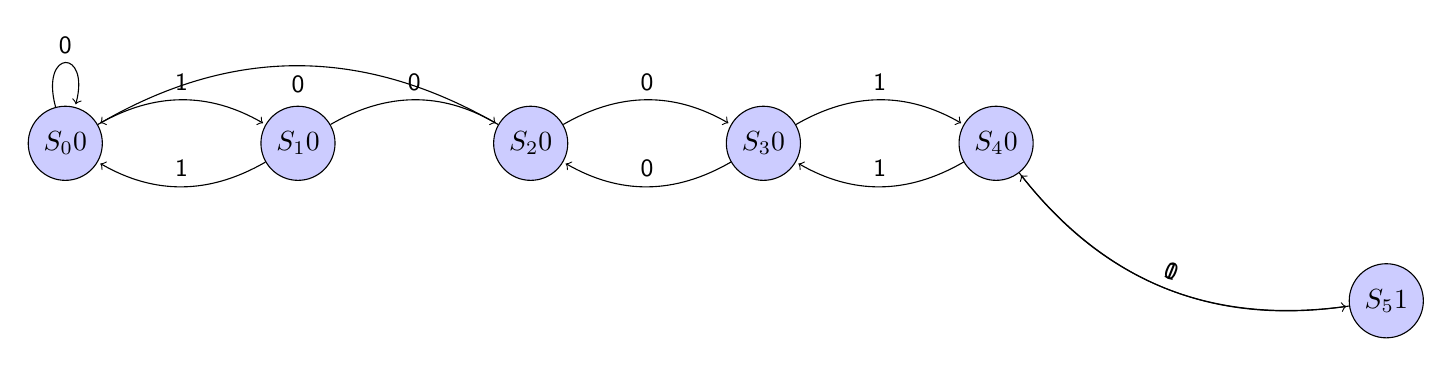
\begin{tikzpicture}[shorten >=1pt,->,node distance=2cm]
    \node[state,fill=blue!20] (S0) {$S_0$ \\ $0$};
    \node[state,fill=blue!20,right=of S0] (S1) {$S_1$ \\ $0$};
    \node[state,fill=blue!20,right=of S1] (S2) {$S_2$ \\ $0$};
    \node[state,fill=blue!20,right=of S2] (S3) {$S_3$ \\ $0$};
    \node[state,fill=blue!20,right=of S3] (S4) {$S_4$ \\ $0$};
    \node[state,fill=blue!20,right=of S4,xshift=2cm,yshift=-2cm] (S5) {$S_5$ \\ $1$};

    \path[every node/.style={font=\sffamily\small}]
        (S0) edge[loop above] node {0} ()
             edge[bend left] node[sloped,above] {1} (S1)
        (S1) edge[bend left] node[sloped,above] {0} (S2)
             edge[bend left] node[sloped,above] {1} (S0)
        (S2) edge[bend left] node[sloped,above] {0} (S3)
             edge[bend right] node[sloped,below] {0} (S0)
        (S3) edge[bend left] node[sloped,above] {1} (S4)
             edge[bend left] node[sloped,above] {0} (S2)
        (S4) edge[bend right] node[sloped,above] {0} (S5)
             edge[bend left] node[sloped,above] {1} (S3)
        (S5) edge[bend left] node[sloped,above] {1} (S4);
\end{tikzpicture}

\end{document}